\subsection{Supported magnitude-frequency distributions}
The magnitude-frequency distributions currently supported by the 
\gls{acr:oqe} are the following: 
\begin{description}
    \item[A discrete incremental magnitude-frequency distribution] \hfill \\
    It's the most versatile distribution supported. It's defined by the 
    minimum value of magnitude (representing the mid point of the first
    bin) and by the bin width. The distribution itself is simply a 
    sequence of floats (or exponentials) describing the annual rate of events for 
    each different bin. Below we provide an example of the xml that should
    be incorporated in order to define this \gls{acr:mfd} for a given
    seismic source.
\begin{Verbatim}[frame=single, commandchars=\\\{\}, fontsize=\footnotesize]
<incrementalMFD minMag="5.05" binWidth="0.1">
    <occurRates>0.15 0.08 0.05 0.03 0.015</occurRates>
</incrementalMFD>
\end{Verbatim}
    The magnitude-frequency distribution obtained with the above
    settings is shown in Figure \ref{fig:evenly_discretized_mfd}.
% ..............................................................................
% . . . . . . . . . . . . . . . . . . . . . . . . . . . . . . . . . . . > Figure
\begin{figure}[!ht]
\centering
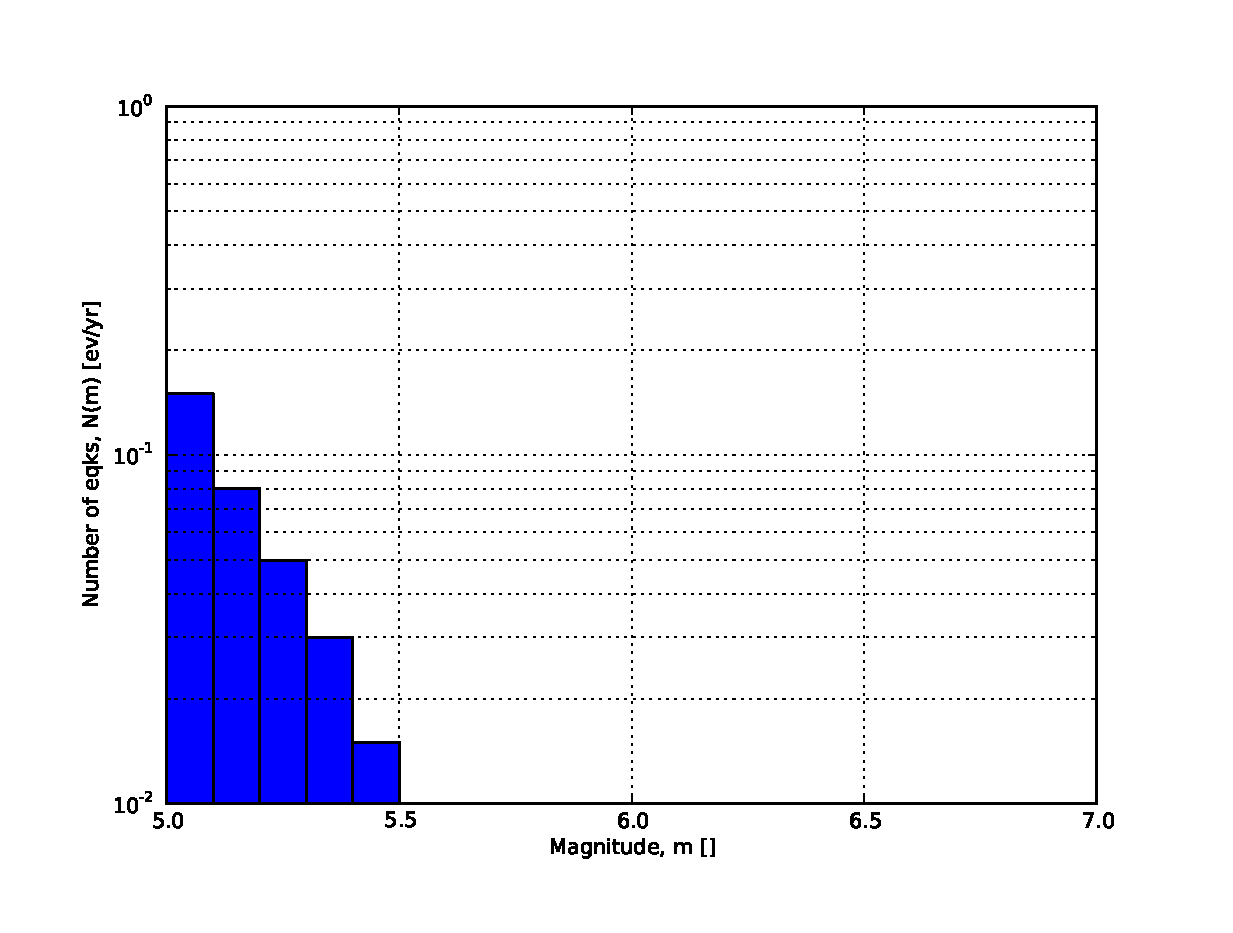
\includegraphics[width=12cm]{./figures/hazard/ed_mfd.eps}
\caption{Incremental magnitude-frequency distribution.}
\label{fig:evenly_discretized_mfd}
\end{figure}
% . . . . . . . . . . . . . . . . . . . . . . . . . . . . . . . . . . . < Figure
% ..............................................................................
%
\item[A double truncated Gutenberg-Richter distribution] \hfill \\
    This distribution is de\-scribed by means of a minimum \texttt{minMag}
    and maximum magnitude \texttt{maxMag} and by the $a$ and $b$ values 
    of the Gutenberg-Richter relationship. The synthax of the xml is 
    rather compact as shown below
\begin{Verbatim}[frame=single, commandchars=\\\{\}, fontsize=\footnotesize]
<truncGutenbergRichterMFD aValue="5.0" bValue="1.0" minMag="5.0" 
        maxMag="6.0"/>
\end{Verbatim}
    The magnitude-frequency distribution obtained using the 
    parameters of the considered example is shown in Figure \ref{fig:dt_gr_mfd}
% ..............................................................................
% . . . . . . . . . . . . . . . . . . . . . . . . . . . . . . . . . . . > Figure
\begin{figure}[!ht]
\centering
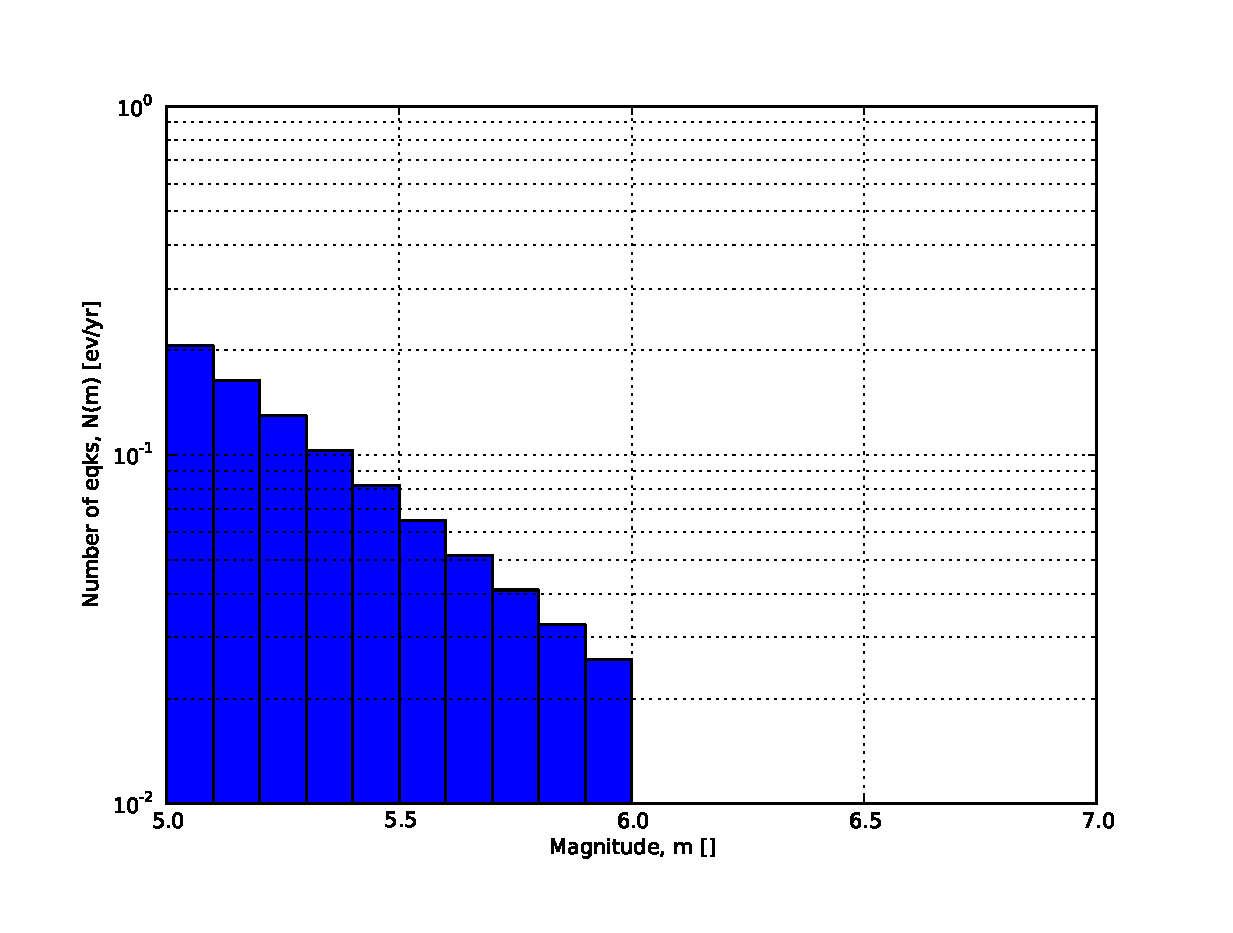
\includegraphics[width=12cm]{./figures/hazard/dt_mfd.eps}
\caption{Double truncated Gutenberg-Richter magnitude-frequency distribution.}
\label{fig:dt_gr_mfd}
\end{figure}
% . . . . . . . . . . . . . . . . . . . . . . . . . . . . . . . . . . . < Figure
% ..............................................................................
%
%
%\item[Characteristic earthquake model (\`{a} la \cite{youngs1985})]
%    In \citexear{youngs1995}, \citeauthor{youngs1995}
%\begin{Verbatim}[frame=single, commandchars=\\\{\}, fontsize=\footnotesize]
%    AA
%\end{Verbatim}
%% ..............................................................................
%% . . . . . . . . . . . . . . . . . . . . . . . . . . . . . . . . . . . > Figure
%\begin{figure}[!ht]
%\centering
%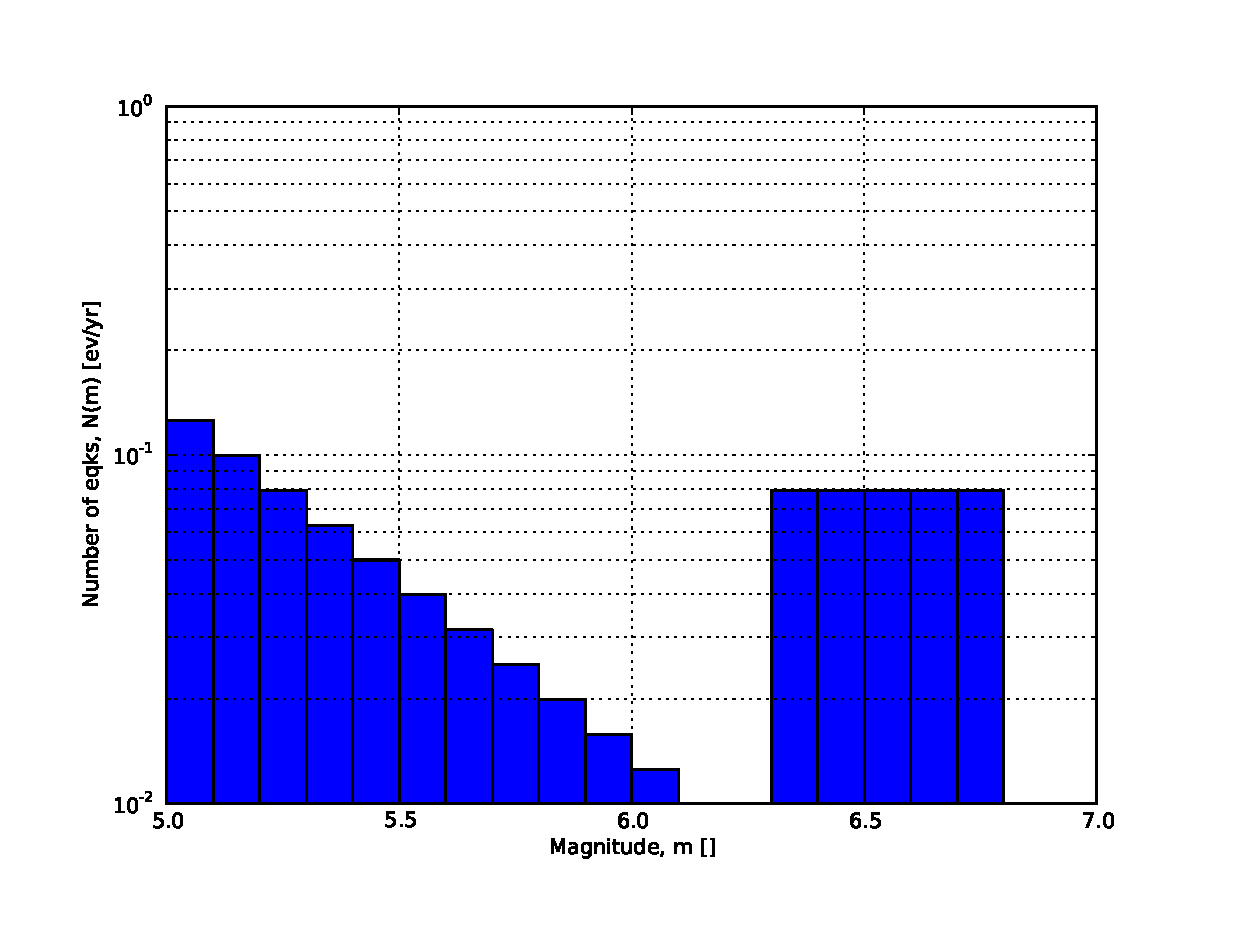
\includegraphics[width=12cm]{./figures/hazard/yc_mfd.eps}
%\caption{\cite{youngs1985} magnitude-frequency distribution.}
%\label{fig:yc_gr_mfd}
%\end{figure}
% . . . . . . . . . . . . . . . . . . . . . . . . . . . . . . . . . . . < Figure
% ..............................................................................

\end{description}
